\documentclass[a4paper, fontsize=14pt]{article}
\usepackage[T2A]{fontenc}
\usepackage{mathtools}
\usepackage[utf8]{inputenc}
\usepackage[english, russian]{babel}
\usepackage{fancyhdr}
\usepackage{graphicx}
\usepackage{gensymb}
\usepackage{floatrow}
\usepackage{titlesec}
\usepackage{lastpage}
\usepackage{float}
\usepackage{gensymb}
\usepackage{booktabs}
\usepackage{amsmath}
\usepackage{amssymb}

\pagestyle{fancy}
	\fancyhf{}
	\lhead{\hspace{1bp} Работа \textnumero 3.2.3}
	\rhead{Мистер Давид Максимович Абрамсон 878\hspace{1bp}}
	\lfoot{Резонанс токов в параллельном контуре}
	\cfoot{\textbf{}}
	\rfoot{\thepage\ \textnormal{из}\ \pageref{LastPage}}
	\renewcommand{\headrulewidth}{1pt}
	\renewcommand{\footrulewidth}{1pt}


%\addtolength{\hoffset}{-1.75cm}
%\addtolength{\textwidth}{3.5cm} 

%\addtolength{\voffset}{-1.5cm}
%\addtolength{\textheight}{3cm} 

\titleformat{\section}
    [block]{\normalfont\bfseries\large}{\rlap{\thesection}}{0em}
    {\vspace{-0.02\textwidth}\begin{minipage}[t]{.95\textwidth}}
[\end{minipage}]

\thispagestyle{fancy}

\begin{document}
\selectlanguage{russian}


\huge
\centering
\textbf{Резонанс токов в параллельном контуре}

\raggedright
\parindent=1cm
\large
	\section*{Цель работы}
 Исследование резонанса токов в параллельном колебательном контуре с изменяемой ёмкостью, включающее получение амплитудно-частотных и фазово-частотных характеристик, а также определение основных параметров контура.
 	\section*{Оборудование}
 Генератор сигналов, источник тока, нагруженный напараллельный колебательный контур с переменной ёмкостью, двулучевой осциллограф, цифровые вольтметры.
	\section*{Экспериментальная установка}
	\begin{figure}[H]
	\includegraphics[width = 1.0\linewidth]{ust.png}
	\caption{Схема экспериментального стенда.}
	\end{figure}
	\section*{Теоретическая часть}
	Схема экспериментального стенда для изучения резонанса токов в параллельном колебательном контуре показана на рисунке 1. Синусоидальный сигнал от генератора  поступает на вход источника тока, собранного на операционном усилителе ОУ с полевым транзистором ПТ, питание которых осуществляется встроенным блоком-выпрямителем от сети переменного тока 220 вольт. Цепи питания на схеме не показаны, представлен только резистор $R_1$, переменное напряжение на котором в используемой схеме равно напряжению на входе <<+>> операционного усилителя. Источник тока, обладающий по определению бесконечным внустренним сопротивлением, фактически обеспечивает потоянство амплитуды тока $I$ на меняющейся по величине нагрузке --- параллельном контуре, изображенном на рисунке 1 в виде эквивалентной схемы. Источник тока, колебательный контур и блок питания заключены в отдельный корпус с названием <<Резонанс токов>> на верхней крышке, отмеченный на рисунке штриховой линией.
	
	На корпусе имеются коаксиальные разъёмы <<Вход>>, <<$U_1$>> и <<$U_2$>>, а также переключатель магазина ёмкостей $C_n$ с указанием номера $n = 1, 2, \ldots 7$. Величины ёмкостей $C_n$ и сопротивления $R_1$, указаны в табличке на крышке корпуса. Напряжение $E = E_0 \cos (\omega t + \phi_0)$ поступает на вход <<+>> операционного усилителя от генератора через согласующую $RC$-цепочку. Это же напряжение через разъём <<$U_1$>> подаётся одновременно на канал 1 осциллографа GOS-620 и вход 1-го цифрового вольтметра GDM-8245. Переменное напряжение на резисторе $R_1$, как отмечалось выше, при этом также равно $E$. Напряжение на контуре $U$, совпадающее с напряжением на конденсаторе, подаётся со знаком <<->> через разъём <<$U_2$>> на канал 2 осциллографа и вход 2-го цифрового вольтметра GDM-8245. Как видно из схемы,
	\[
		I = E / R_1 = I_0 \cos (\omega t + \varphi_0), \quad I_0 = E_0 / R_1.
	\]
	Активные потери в конденсаторе, пропорциональные, как известно, косинусу угла $\varphi$ сдвига фаз между током и напряжением на ёмкости, убывают с ростом $\varphi$ и, соответственно, с уменьшением угла $\delta = 90\degree - \varphi$. Потери в конденсаторе принято характеризовать величиной $\tg \delta$, обычно приводимой в документации к изделию. Из закона Ома получаем выражение для эквивалентного последовательного напряжения (ЭПС) на циклической частоте $\omega = 2 \pi f$ в виде
	\[
	R_S = \frac{U_{RS}}{I} = \frac{U_{RS}}{\omega C U_{CS}} = \frac{1}{\omega C} \tg \delta.
	\]
	В индуктивную ветвть параллельного колебательного контура нашей установки добавлен постоянный резистор $R$, несколько снижающий его добротность. Это сделано для упрощения процедур получения и обработки резонансных кривых. Таким образом, суммарное активное сопротивление контура при его последовательном обходе принимается равным
	\[
		R_\Sigma = R_L + R + R_S.
	\]
	Далее будем пользоваться методом комплексных амплитуд. Для импедансов Ёмкостной $Z_C$ и индуктивной $Z_L$ ветвей контура получаем формулы:
	\[
		Z_C = R_S - \frac{i}{\omega C}, \quad Z_L = R + R_L + i \omega L.
	\]
	Комплексные амплитуды токов в ёмкостной $\vec I_C$ и индуктивной $\vec I_L$ ветвях контура, а также напряжения $\vec U$ на контуре при нулевой начальной фазе $\varphi_0$ внешнего тока $\vec I = I_0 e^{i \varphi_0}$ удобно пеерписать в виде:
	\[
	\vec I_C = \vec I \frac{Z_L}{Z_C + Z_L} = iQI_0 \frac{\omega}{\omega_0} \frac{1 - i \frac{R + R_L}{\rho} \frac{\omega_0}{\omega}}{1 + iQ (\frac{\omega}{\omega_0} - \frac{\omega_0}{\omega})},
	\]
	\[\vec I_L = \vec I \frac{Z_C}{Z_C + Z_L} = -iQI_0 \frac{\omega_0}{\omega} \frac{1 + i \tg \delta}{1 + iQ(\frac{\omega}{\omega_0} - \frac{\omega_0}{\omega})},
	\]
	ЗДесь использованы стандартные обозначения характеристик колебательного контура: $\omega_0 = 1 \ \sqrt{LC}$ --- собственная частота, определяемая из условия $Im (Z_C + Z_L) = 0$, то есть из условия действительности импеданса контура при его последовательном обходе, $\rho = \sqrt{LC}$ --- реактивое, или волновое, сопротивлене, $Q$ --- добротность колебательного контура, связанная с его параметрами соотношениями
	\[
	Q = \rho / R_\Sigma = \omega_0 L / R_\Sigma = 1/\omega_0 C R_\Sigma \gg 1.
	\]
	\newpage
\section*{Обработка результатов измерений}
	\begin{figure}[H]
	\begin{floatrow}
		\ttabbox{\caption{Данные при $C_3$}}{
		\begin{tabular}{|c|c|}\hline
 $U,\ \text{мВ}$ & $f,\ \text{кГц}$ \\\hline
700 &  22.876 \\\hline
750 &  22.953 \\\hline
800 &  23.025 \\\hline
850 &  23.092 \\\hline
900 &  23.194 \\\hline
950 &  23.220 \\\hline
1000 &  23.278 \\\hline
1050 &  23.350 \\\hline
1100 &  23.426 \\\hline
1150 &  23.642 \\\hline
1159 &  23.590 \\\hline
1100 &  23.782 \\\hline
1050 &  23.855 \\\hline
1000 &  23.927 \\\hline
950 &  23.996 \\\hline
900 &  24.058 \\\hline
850 &  24.126 \\\hline
800 &  24.196 \\\hline
750 &  24.273 \\\hline
700 &  24.353 \\\hline
\end{tabular}}
\ttabbox{\caption{Данные при $C_5$}}{
\begin{tabular}{|c|c|}\hline
 $U,\ \text{мВ}$ & $f,\ \text{кГц}$ \\\hline
500 &  19.044 \\\hline
550 &  19.148 \\\hline
600 &  19.240 \\\hline
650 &  19.329 \\\hline
700 &  19.414 \\\hline
750 &  19.504 \\\hline
800 &  19.616 \\\hline
831 &  19.751 \\\hline
800 &  19.890 \\\hline
750 &  19.993 \\\hline
700 &  20.086 \\\hline
650 &  20.157 \\\hline
600 &  20.249 \\\hline
550 &  20.324 \\\hline
500 &  20.403 \\\hline
\end{tabular}}
\end{floatrow}
\end{figure}

Построим АЧХ для двух ёмкостей $C_3$ и $C_5$:
 \begin{figure}[H]
	\caption{График в координатах $f, U(f)$}
	\center
	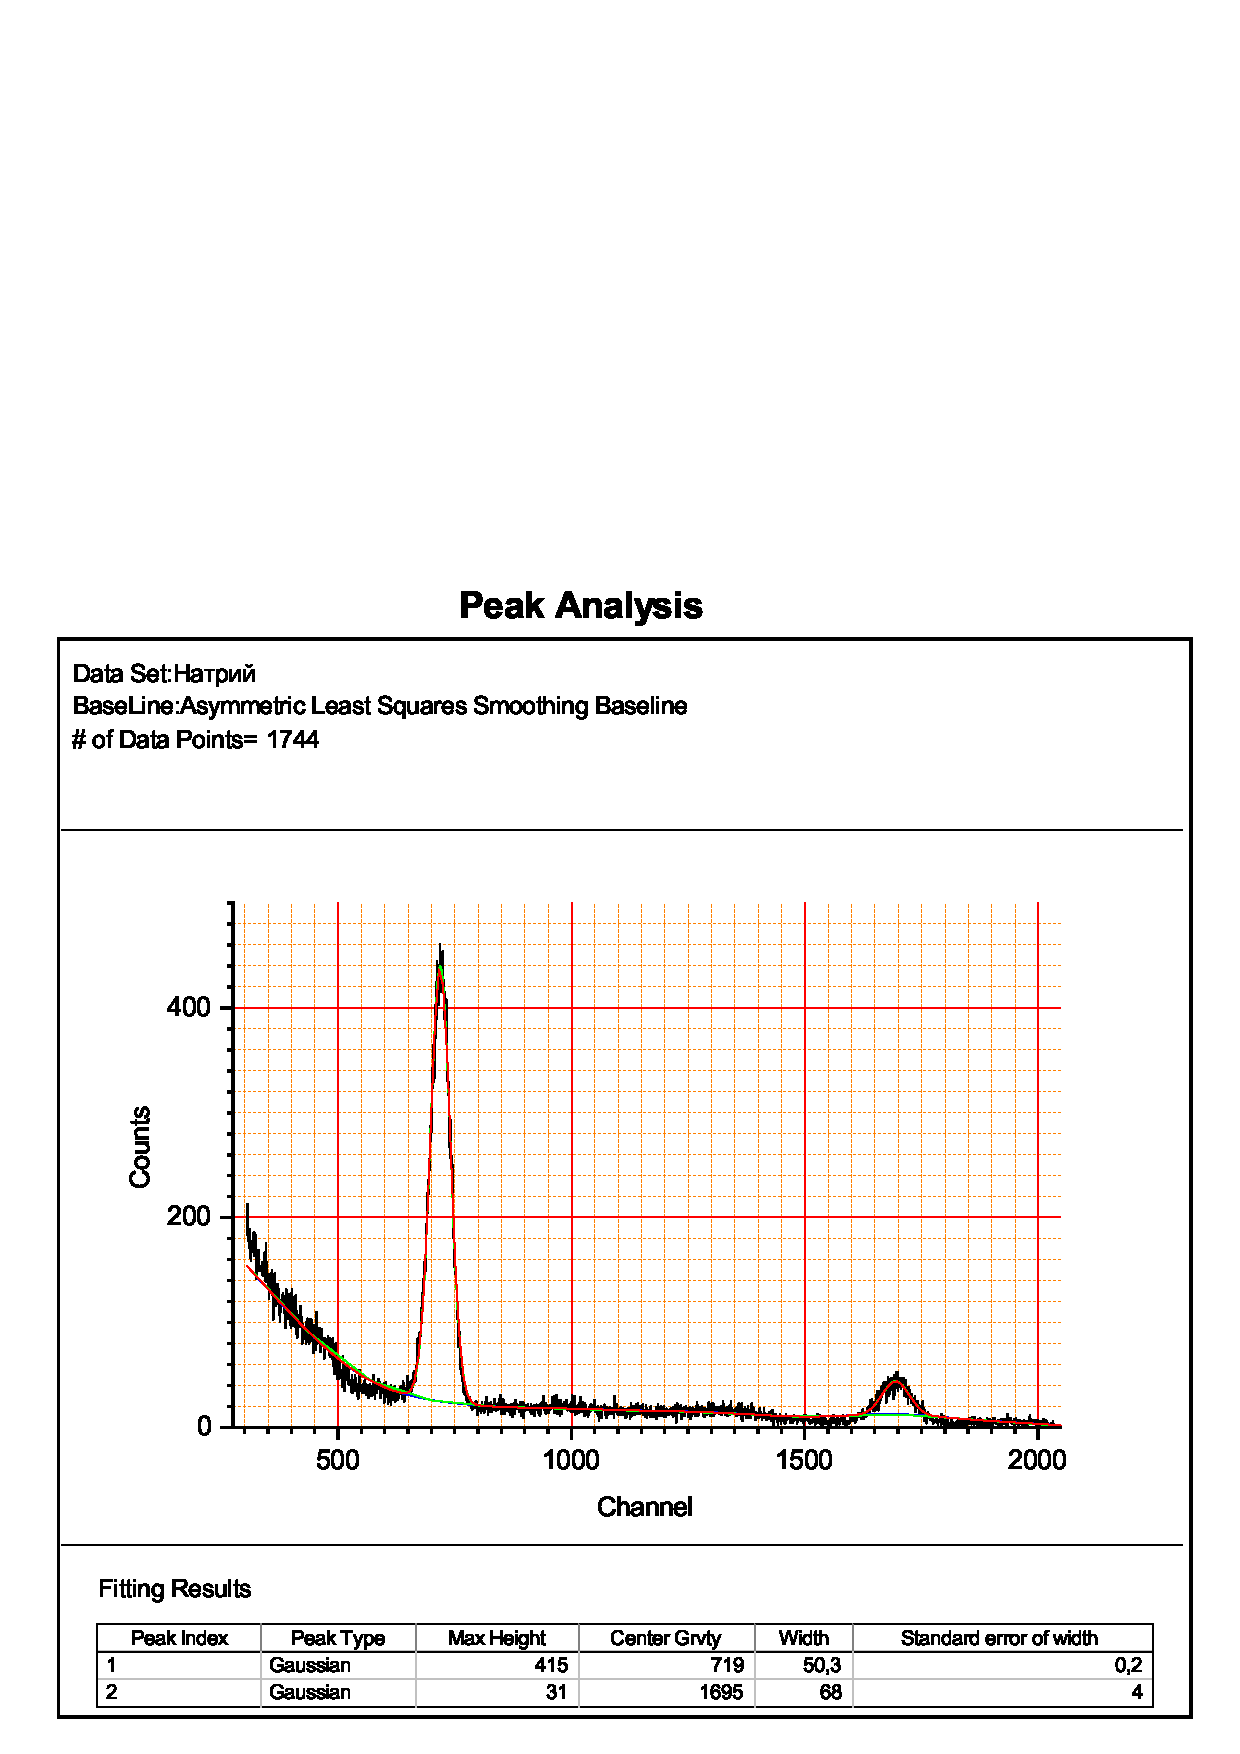
\includegraphics[scale=0.4]{1.jpg}
\end{figure}
 \begin{figure}[H]
	\caption{График в координатах $f/ f_\text{рез}, U(f) / U(\text{рез})$}
	\center
	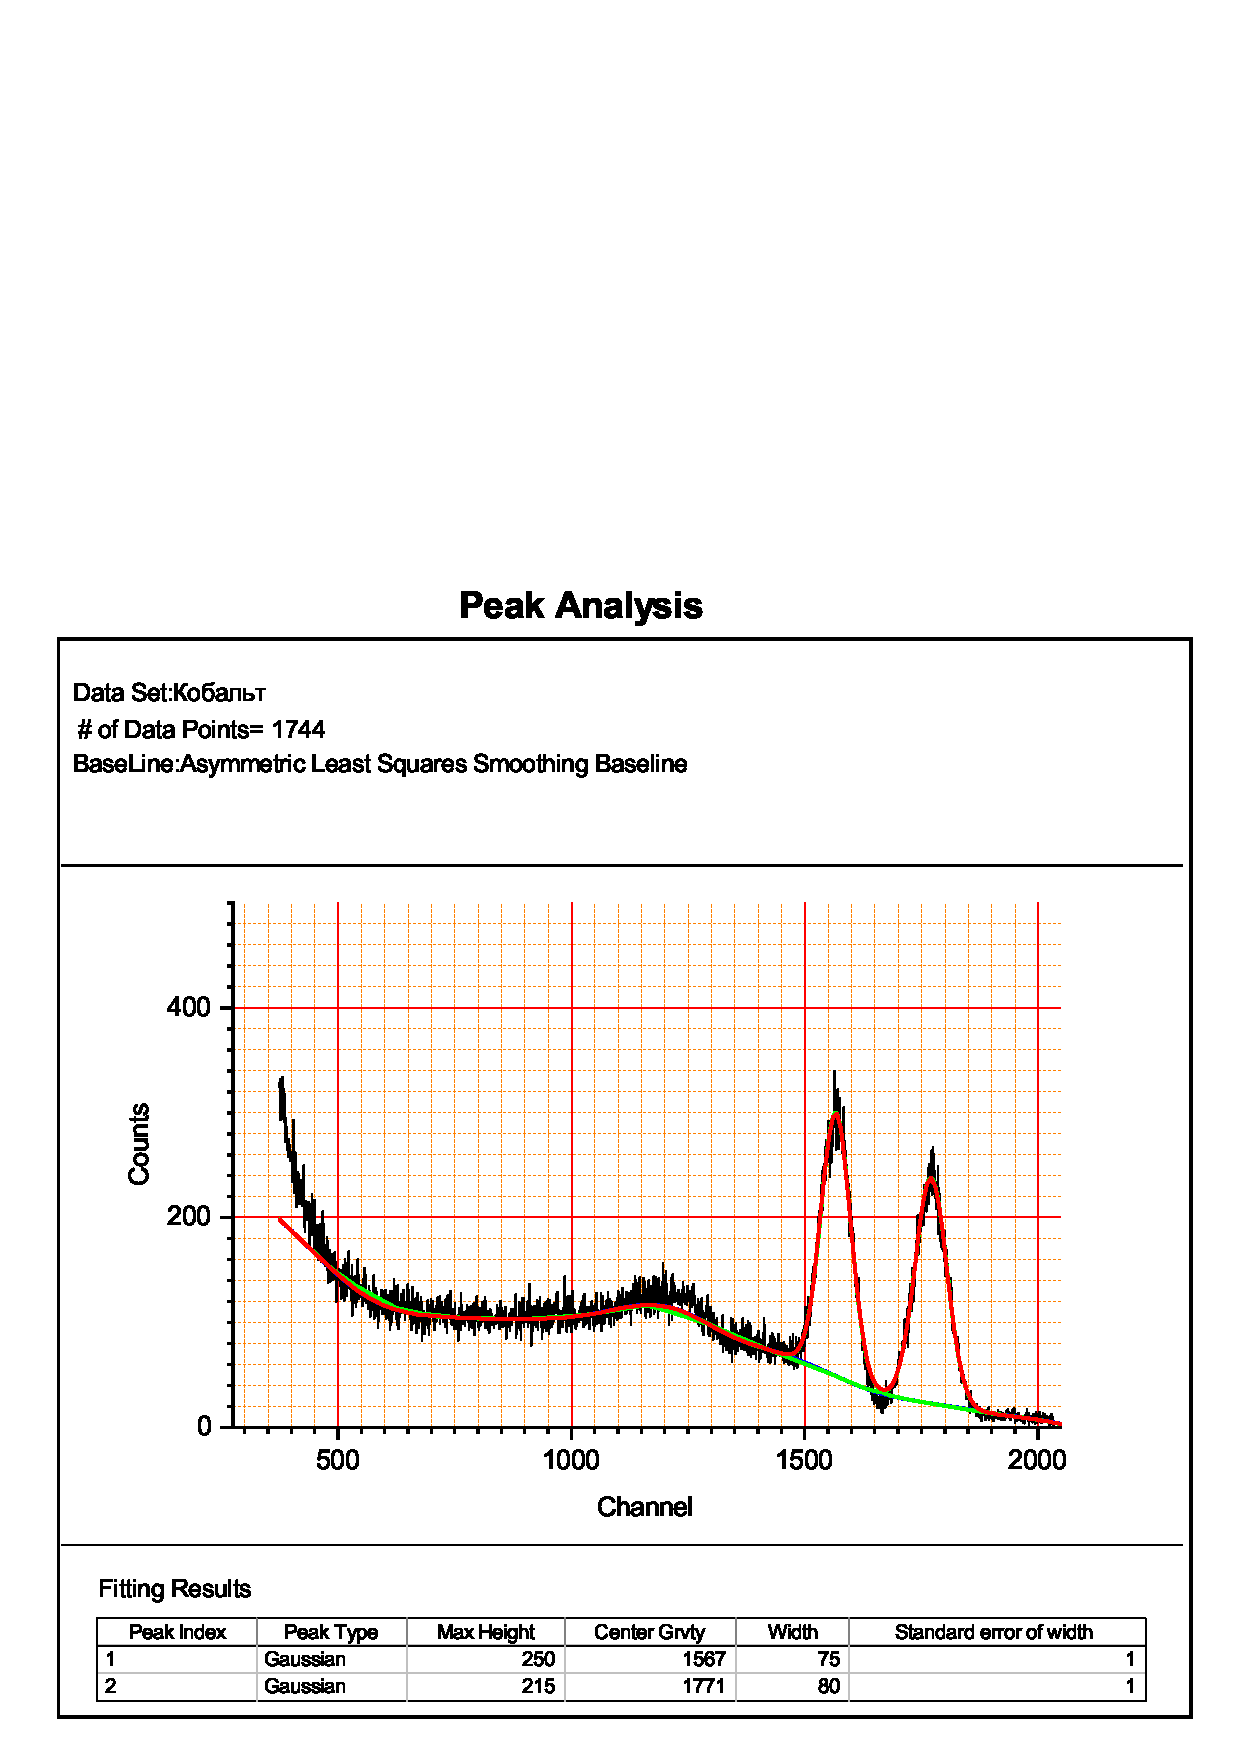
\includegraphics[scale=0.4]{2.jpg}
\end{figure}
По ширине резонансной кривой определим добростность:
\[
Q_1 = 9; \quad Q_2 = 34;
\]
 \begin{figure}[H]
	\caption{Результирующая таблица}
	\center
	\includegraphics[scale=0.6]{res.png}
\end{figure}
\section*{Вывод}
В этой лабораторной работе мы исследовали резонанс колебательного контура, возникающий при слвпадении собственной частоты колебаний и внешней частоты. В идеальном контуре при резонансе колебания бы продолжались бесконечно, но в реальности из-за неидеальности элементов колебательного контура колебания угасают, что и характеризует такой параметр контура, как добротность.
\end{document}